\chapter{Requirements of Intention-oriented Organizational Modeling}
\label{chap:analysis}
This chapter positions the thesis work in the field of process modeling with respect to other existing approaches. The first section provides a detailed requirement analysis of intention-oriented organizational modeling. The last section provides a detailed literature review about the existing approaches. A detailed evaluation of the existing approaches with the proposed requirements is also provided in the last section.

%%%%%%%%%%%%%%%%%%%%%%%%%%%%%%%%%%%%%%%%%%%%%%%%%%%%%%%%%%%%%%%%%%%%%%%%%
\section{Requirement Analysis of Intention-oriented Organizational Modeling}
\label{sec:requirementssupoorting}
%%%%%%%%%%%%%%%%%%%%%%%%%%%%%%%%%%%%%%%%%%%%%%%%%%%%%%%%%%%%%%%%%%%%%%%%%
The requirements of intention-oriented organizational modeling has been derived from the existing literatures \cite{McManus2007, Mandic2010,Bleistein2006, Lacom, Brambilla2012} and from the motivating scenario described in Chapter \ref{chap:motivatingScenario}. 

\subsection{Organizational Intention Transparency (R1)}
An intention can be broken down into definitive actionable components upon which individual resources can act. When these lower level intentions are made achievable for individual resources, then they can be combined to provide successful execution of higher level intention, i.e., main intention. This requires privilege for different organizational members to observe lower level and higher level intentions. Additionally, intentions should also be traceable from different levels of the organizational hierarchy. This means that the status of each intention can be accessed by members in different levels of the organizations. This level of transparency within an organization reduces inefficiencies during intention execution and is a key factor in attracting and retaining high performers in the labor market \cite{McManus2007}. Requirement R1 has to be satisfied in the modeling phase itself as the designing of intentions, strategies and their recursive structures are done during the modeling phase. The prerequisites to satisfy this requirement are, intentions can be refinable and organizational members can view intentions at different levels. 

\subsection{Organizational Strategy-based Cost Estimation (R2)}
Linking strategies with capabilities that has matching resource enable us a cost estimation for each strategy. This is because, strategies are associated with organizational capabilities which in turn are associated with organizational resources. The cost of organizational resources is known, which can be expressed in terms of usage per hour. To incorporate the cost estimation of strategies, we have to understand the recursive structure of the strategies associated with process definitions and then with the resource definitions. Further on, the cost of a strategy can be analyzed using the costs of derived process definitions and then with resource definitions. Including resources cost in strategy cost calculation is important. This is achieved by associating resource models' cost with process models' cost. The recursion is stopped when each resource definition is associated with cost. At the moment an intention is achieved, some resources should be allocated through strategy to maintain the desired state \cite{Mandic2010}. This helps business experts in making resource selection based on strategy cost during modeling itself. For example, if resource is associated with a certain cost then this cost is considered for strategy implementations cost calculation based on which cost to achieve an intention through a strategy is calculated. This type of cost calculation based on intention model is estimated cost of an intention. The cost of an intentions's instance, is the actual cost of an intention. Since intentions are achieved through strategy we should also be able to calculate cost of intention based on cost of its strategies. Allocation of resources is mainly done at the operational level, hence requirement R2 has to be satisfied during the modeling phase. The prerequisites to satisfy this requirement are resources associated with cost and strategy cost estimation that includes all recursive structure.

\subsection{Organizational Strategy Achievability Estimation (R3)}
 The validity of an organizational strategy is assured when the strategy is associated with valid capabilities. A capability can be considered as a valid capability when there exist organizational resources providing the capability. A valid strategy can be implemented as independent informal process. When low level strategies are achievable, then it can be used to estimate the achievability of the higher level strategies. This enables validation of strategic alignment of strategies' recursive structure, i.e., as a sequence of valid strategies \cite{Bleistein2006}. Requirement R3  can be done during the modeling phase of the process as strategy achievability estimations are done before starting the execution of the process. For a strategy to be achieveable the required prerequisites are, strategy should be associated with a valid capability which has organizational resources providing the capability and strategy can be implemented as independent informal process.
 
\subsection{Intention Oriented Working Style (R4)}
As each member of the organization is aware of the higher level and lower level intentions, an organizational member can engage for explicit intentions. Intention orientation is the degree, to which a person or an organization inclined and work towards achievement of an intention. Strong intention orientation advocates that focus on a task is more. Such a focused task ends in a result that is favorable to both employees and organization. Those with strong intention orientation will be able to accurately judge the effects of reaching the intention as well as the ability to fulfill that particular intention with current resources and skills \cite{Lacom}. Hence we associate processes and resources implicitly with intentions through strategies which enables people to work towards certain intentions. The distinction between explicit knowledge of each low level intention should not be seen as a division but rather as a continuum which aligns towards achieving the higher level intention. Though requirement R4 seems to be part of requirement R1, R4 happens during modeling phase and could also happen during execution phase due to the dynamic nature of informal process. The prerequisites for this requirement are satisfaction of R1 and organizational members requiring understanding of the intentions and how they can be reached.  

\subsection{Participative Organizational Modeling (R5)}
 Different members of an organization participate to create organizational intentions, as a result organizational models are shaped based on input provided by different members of the organization but directed by the executives. The social involvement of different members in a business process model can be regarded as a process optimization phase, where the organization seeks efficiency by extending the reach of a business process to a broader class of people \cite{Brambilla2012}. Since, the requirement is about participative modeling of different groups of people, we also need means to specify different groups of people with different privileges, e.g., view, edit, follow, etc., for accessing different entities such as intentions, strategies, contexts, etc. Since, the requirement itself is about developing models based on input from different organizational members, the requirement has to be satisfied during modeling phase. The prerequisites to satisfy this requirement are satisfaction of R1 and intention-oriented organizational modeling has to be done based on the input provided by different members of the organization.  
 
 The requirement satisfaction phases and the prerequisites to satisfy each requirement are provided in the Table \ref{tab:subrequirements}:

\begin{table} [htbp]
	\centering
	\begin{tabular} {p{2.5cm}p{3cm}p{8cm}}
		\toprule
		\textbf{Requirement} & \textbf{Requirement Satisfaction Phases} & \textbf{Pre-requisites}    \\
		\midrule                                                                                                               
		R1    & Modeling phase    &(1) Main intention can be refinable, (2) Organizational members can view the intentions at different levels.    \\ 
		
		R2   & Modeling phase    &(1) Resources associated with cost, (2) Strategy cost estimation that includes all recursive structure. \\         
			
		R3   & Modeling phase       &(1) A valid capability which has organizational resources providing the capability, (2) Strategies can be implemented as independent informal process. \\      
		
		R4   & Modeling and Execution phases     &(1) Satisfaction of R1, (2) Organizational members require understanding of the intentions and how they can be reached. \\                         
			
		R5  &Modeling phase  &(1) Satisfaction of R1, (2) Intentions has to be modeled based on the input provided by different members of the organization.               \\ 
		    
		\bottomrule
	\end{tabular}
	\caption{Requirements Analysis}
	\label{tab:subrequirements}
\end{table}

%%%%%%%%%%%%%%%%%%%%%%%%%%%%%%%%%%%%%%%%%%%%%%%%%%%%%%%%%%%%%%%%%%%%%%%%%
\section{Literature Review and Evaluation of Related Work}
\label{sec:literaturereview}
%%%%%%%%%%%%%%%%%%%%%%%%%%%%%%%%%%%%%%%%%%%%%%%%%%%%%%%%%%%%%%%%%%%%%%%%%
In the literature, several work has been done in order to support and automate the business processes such as strategy-driven \cite{Bider2005}, activity-centric\cite{Yarosh2009}, activity-oriented \cite{Leymann2000}, artifact-centric \cite{Cohn2009}, capability-driven \cite{Stirna2012} and ArchiMate \cite{Group2012}. This section provides, a detailed description about these approaches and evaluation of these approaches based on requirements mentioned in the Section \ref{sec:requirementssupoorting}. 

\subsection{Strategy-driven} 
Strategy driven approach is a decision oriented modeling approach that focus on goals of the processes and refine goals until the operational level. This approach defines business process in terms of goals and strategies in order to achieve the goals. It also uses map representation system that contains goals and strategies. In this approach, goals are refinable and it recognizes concept of goals (intentions) during modeling. Thus, this approach satisfies both the prerequisites of requirement R1. The details about cost of a resource and strategy cost calculation is not addressed. Hence, requirement R2 is not satisfied as both of its prerequisites are not met. The approach does not provide any information about the capability and association of a capability with a resource. Thus, the first prerequisite of requirement R3 is not met. Also, the approach does not provide any information regarding the execution of a strategy as an independent informal process. Thus, second prerequisite of requirement R3 is also not met. So, the requirement R3 is not satisfied by the approach. Requirement R4 is satisfied, as it satisfies R1 and this approach also requires understanding of goals by the organizational members. The requirement R5 is partially satisfied, as the approach satisfies requirement R1. But another prerequisite, i.e., intentions has to be modeled based on the input provided by different members of the organization to satisfy R5 is not addressed by the approach. 

\subsection{Activity-oriented} 
Traditional business process modeling techniques such as BPMN \cite{bpm2011}, BPEL \cite{Std.2007}, etc., are activity-oriented process models and executed based on these models. Requirements R1, R4 and R5 are not satisfied as details of modeling based on intentions are not provided because the approach itself is activity-oriented. The information about cost of achieving a strategy is not mentioned. Due to the lack of concrete cost calculation method in activity-oriented approach, there are integrated modeling or complementary modeling approaches \cite{Bankhofer2013,Sampathkumaran2013} proposed to support cost calculation based on resource. Thus, first prerequisite of requirement R2 is satisfied. The second prerequisite, i.e., strategy cost estimation that includes all recursive structure, is not addressed by the approach. Thus, requirement R2 is partially satisfied. Since, both the prerequisites of requirement R3 are not met, the requirement R3 is also not satisfied by the approach. 

\subsection{Activity-centric} 
The activity-centric approach also supports knowledge workers by providing shared activity constructs (i.e., activity-oriented constructs) as a computational unit for organizing the work. Though this approach provides team level view of past and ongoing work by supporting propagation of completed activities to the existing activities, the approach is not intention-oriented. Thus, requirements R1, R4 and R5 are not met as the approach itself is activity-centric. The details about cost calculation is not addressed. Thus, requirement R2 is not satisfied as both the prerequisites are not satisfied. The prerequisites of requirement R3 are not addressed by the approach. Thus, requirement R3 is also not satisfied.   
 
\subsection{Artifact-centric} 
Artifact-centric is a data-centric approach to model business processes based on business relevant data. The artifact-centric approach combines business data (artifacts) and business process in a holistic way. Requirements R1, R4 and R5 are not satisfied as details of intentions and modeling based on intentions are not provided as the approach itself is artifact-centric. The requirement R2 which is about cost calculation is also not addressed. The prerequisites of requirement R3 were not addressed by the approach. Hence, requirement R3 is also not satisfied. 

\subsection{Capability-driven} 
The capability-driven approach also proposes to support the changing environment of organizations. This approach aims to aid development of business models by connecting goals and capabilities. The requirement R1 is satisfied by the approach, as it satisfies both the prerequisites related to intentions. This approach claims that, it overcomes the challenge of high cost in developing applications but there is no clear details about how cost calculation is done, hence requirement R2 is not addressed. In this approach, capabilities and resources can be associated. Thus, it satisfies the first prerequisite of requirement R3. The second prerequisite, i.e., strategies can be implemented as independent informal process is not addressed by the approach. Thus, requirement R3 is partially satisfied. The first prerequisite for requirement R4 is satisfied and second prerequisite is also satisfied by the approach. Thus, requirement R4 is satisfied by the approach. The first prerequisite for requirement R5 is satisfied and second prerequisite is not addressed by the approach. Thus, requirement R5 is also partially satisfied. 

\subsection{ArchiMate}
ArchiMate provides an integrated modeling approach by allowing to model based on both activities, i.e., business process and business functions such as knowledge, resources, etc. ArchiMate allows modeling based on goals and provides visibility of whole process, supports viewpoints in different levels of modeling. Thus, requirement R1 is addressed. ArchiMate does cost calculation based on goals and resources. Thus, requirement R2 is partially satisfied, because cost calculation details regarding the strategy that includes all recursive structure is not provided.  In this approach, capabilities and resources can be associated. Thus, it satisfies the first prerequisite of requirement R3. The second prerequisite is also satisfied by the approach, because strategy models can be implemented through this approach. Thus, requirement R3 is satisfied by the approach. Requirement R4 is satisfied because both the first and second prerequisites are satisfied. Similarly, requirement R5 is also satisfied because the approach satisfies first and second prerequisites.  

\subsection {Summary of the Evaluation}
 The Table \ref{tab:evaluationoftheapproach}, shows the evaluation of related works based on the derived requirements. From the table one could comprehend that none of the evaluated approaches satisfy all the requirements together. Thus, we propose a new intention-oriented organizational modeling approach in the Section \ref{sec:topdownapproach} of Chapter \ref{chap:approach} that satisfies all of the derived requirements of intention-oriented organizational modeling. 

 \begin{table}
 	\centering
 	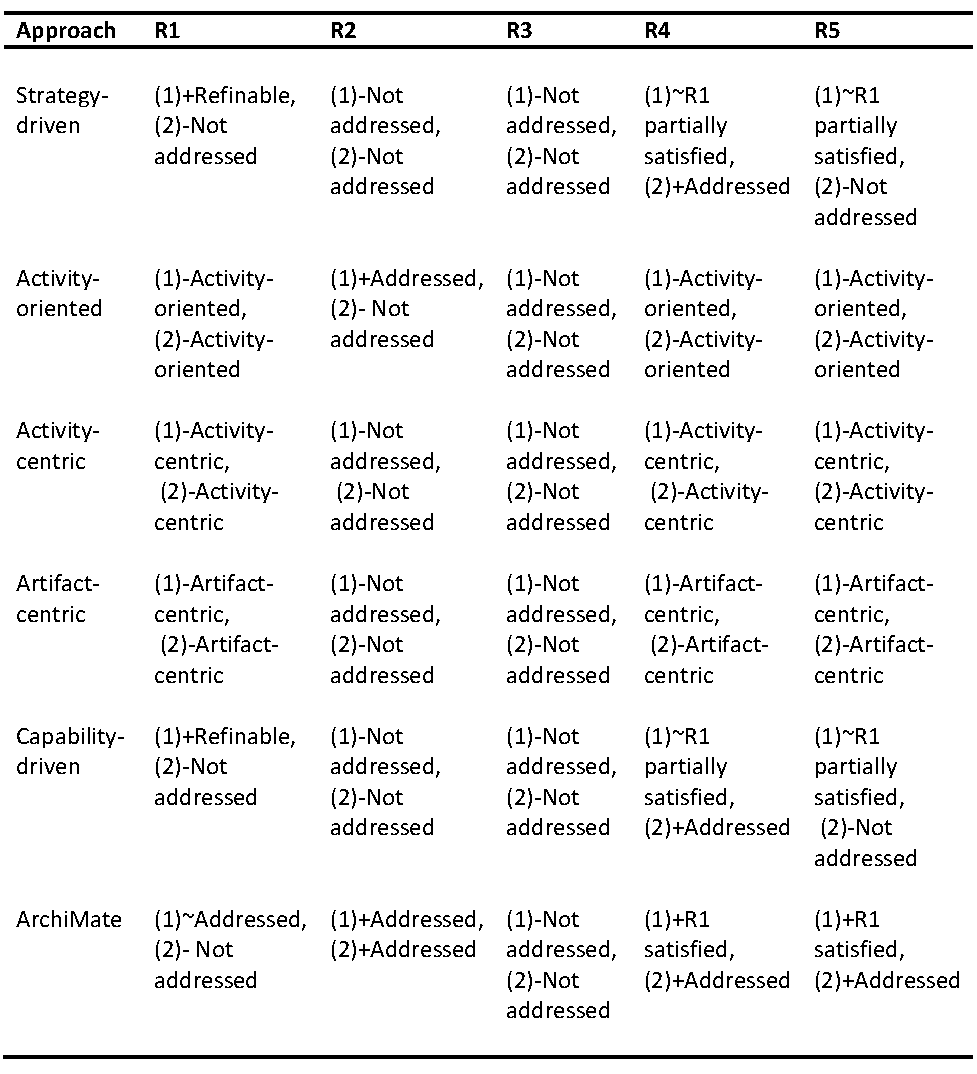
\includegraphics[width= \textwidth]{Approach.pdf}
 	\caption{Summary of the Evaluation}
 	\label{tab:evaluationoftheapproach}
 \end{table} 


